\documentclass{article}
\usepackage[utf8]{inputenc}
\usepackage{amsmath,amssymb}
\usepackage{pgfplots}

\newcommand{\calG}{\mathcal{G}}


\title{Physics 708: Statistical Mechanics}
\author{Dion O'Neale 
	and Nicola Gujer
	and another person}
\begin{document}
\maketitle
\section*{Thermodynamics - a refresher}
We'll start with a quick overview of some of the important concepts from classical thermodynamics. These ideas motivated much of statistical mechanics. This section will also recap some content from 315.

\subsection*{Macroscopic laws of thermodynamics}
In thermodynamics we study a system --- the part of the world that we are interested in --- that is separated from its surroundings --- the rest of the universe --- by some boundary.

We can classify the types of systems into three types based on the type of walls that define the system boundary:
\begin{itemize}
\item Adiabatic walls/isolated system - no energy or matter is transferred
\item Diathermal walls/closed system - no matter can be transfered but heat can flow through the walls.
\item (semi-)permeable walls/open system - in addition to heat, one or more chemical species can be transfered through the walls. 
\end{itemize}

\subsection*{The four laws of thermodynamics}
Only four laws are required to construct the relationships that control much of classical thermodynamics. Theses are, in brief:
\begin{itemize}
\item {\bf Zeroth law} Defines temperature and thermal equilibrium.
\item {\bf First law} Formulates the principle of conservation of energy for thermodynamic systems. (Energy is conserved)
\item {\bf Second law} Entropy increases; heat spontaneously flows from high to low temperatures.
\item {\bf Third law} The absolute zero of temperature is not attainable.  
\end{itemize}


We'll revisit the first two laws in a bit more detail and then make use of the second law to derive some familiar properties of heat.

\subsection*{Zeroth law:}
If two systems are each in thermal equilibrium with a third system, then they are in thermal equilibrium with each other. This implies that they have some property in common. We call this property \emph{temperature}. (In the language of mathematics, thermal equilibrium is a transitive property.)

It is worth noting that thermal equilibrium is not the same as thermodynamic equilibrium. For the latter we also need mechanical equilibrium ($p_1=p_2$) and chemical equilibrium ($\mu_1=\mu_2$ --- equal rates of reaction).

\subsection*{First Law:}
Energy remains constant for a (collection of) system(s) isolated from the surroundings. When a system interacts with its surroundings any increase in the energy of the system is equal to the work done on the system by the surroundings. (We denote work done \emph{on} the system as $W>0$, similarly, heat supplied to the system is denoted $Q>0$.)

When considering the change in energy $\Delta E$ of a system it is necessary to consider both work and heat.

E.g. System $A$ gains energy from system $B$, i.e. $\Delta E_A = -\Delta E_B \implies \Delta E_A + \Delta E_B =0$. But, in general, $\Delta E_A\neq W_{B\rightarrow A}$ since there can also be a heat flow $Q_{B\rightarrow A}$ due to a temperature difference.
So,
$$\Delta E_A = W_{B\rightarrow A} + Q_{B\rightarrow A}$$
$$\Delta E_B = W_{A\rightarrow B} + Q_{A\rightarrow B}.$$

Energy conservation gives 
$$\underbrace{(W_{A\rightarrow B}+W_{B\rightarrow A})}_{\text{Work done by the composite system}} + \underbrace{(Q_{A\rightarrow B}+Q_{B\rightarrow A})}_{\text{Heat flow in the composite system}} = 0$$

In an adiabatic (isolated) system the fist law gives a sort of balance sheet for energy/work/heat:
$W_{A\rightarrow B}+W_{B\rightarrow A} = 0$ and $Q_{A\rightarrow B}+Q_{B\rightarrow A}$.

Revision: Adiabatic work and heat flow. Quasi-static processes (how slow is slow enough?). Path dependence of work.
 - see the notes from 315 that are in the repository. You may want to incorporate the relevant content from those notes, or other sources, into this document.


The \emph{internal energy} of a system is the energy associated with the internal degrees of freedom of the system. If a system is at rest and the potential energy of any external field is unimportant, then the internal energy of a system is the total energy of a system.

The equation of state for internal energy is usually written $E = E(T,V,N)$ or $E = E(T,P,N)$. Expressing these as infinitesimals (change in internal energy) gives
$$ dE = \frac{\partial E}{\partial T}\bigg\vert_{V,N}dT + \frac{\partial E}{\partial V}\bigg\vert_{T,N}dV +\frac{\partial E}{\partial N}\bigg\vert_{T,V}dN$$
a similarly, for the second formulation.

Note $ \frac{\partial E}{\partial T}\vert_{V,N} \neq \frac{\partial E}{\partial T}\vert_{P,N} $

\subsection*{Heat capacity:}
Heat flowing into a system causes a change in temperature (except in the case of phase transitions). $T\rightarrow T=\Delta T$. The heat capacity of a system depends, in part on the experimental conditions of the system under consideration. Two important cases are constant volume and constant pressure.

For constant volume we have
$$C_V = \frac{\delta Q}{dT}\bigg\vert_V$$
similarly, for constant pressure,
$$C_P = \frac{\delta Q}{dT}\bigg\vert_P.$$

The first law of thermodynamics (conservation of energy) implies that $\delta Q = dE - \delta W = dE + PdV$  (since $W = Fdx$ and $F=PA \implies W = PdV$). So
$C_V = \frac{\delta Q}{\partial T}\vert_{V,N} = \frac{\partial E}{\partial T}\vert_{V,N}$ (since $dV=0$ for fixed V.)
In the constant pressure case $C_P = \frac{\delta Q}{dT}\vert_{P,N} = \frac{\partial E}{\partial T}\vert_{P,N} + P\frac{\partial V}{\partial T}\vert_{P,N}$.

Constant pressure heat capacity implies that there is a change in volume, so think about how the volume changes. Define the \emph{volumetric thermal expansivity} $\alpha_p = \frac{1}{V}\frac{\partial V}{\partial T}\vert_{P,N} \implies V\alpha_p =\frac{\partial V}{\partial T}\vert_{P,N}$.

We can now write $C_P = \frac{\partial E}{\partial T}\vert_{P,N} + \alpha_pPV$.

An alternative way of thinking about $C_P$: constant pressure implies that $PdV = d(PV)$ so that $\delta Q = dE + \underbrace{dPV}_{=dW} = d(E+PV)$. We define the composite quantity $E+PV$ as \emph{enthalpy}, H, with the equation of state $H = H(T,P,N)$.

The infinitesimal for enthalpy is $dH = \underbrace{dE +PdV}_{\delta Q}+ VdP = \delta Q + VdP\vert_{P}$. The last term is zero, since $P$ is constant, so we get $C_P = \frac{\delta Q}{\partial T}\vert_{P,N} = \frac{\partial H}{\partial T}\vert_{P,N} $.

\subsection*{Intensive and extensive variables}

Intensive variables control the state of a system but are independent of the system size. E.g. $T,P$ (magnetic field?)

Extensive, or additive, variables are proportionate to the size of a system (i.e. they depend on $N$).

It is possible to turn an extensive variable into an intensive variable by normalising by the system size. I.e. the variables come in dual pairs, e.g. pressure and volume.

One important extensive variable is the entropy (or disorder) of a system. The dual variable is temperature.

The intensive variable is the derivative of the internal energy with respect to the corresponding extensive variable given all other extensive variables are held constant. For example, $T = \frac{\partial E}{\partial S}\vert_{V,N}$.

Given two systems 1 and 2, an extensive variable for the composite system $1\cup2$ can be found by simply adding the individual extensive variables. E.g. $N_{1\cup2} = N_1 + N_2$, $V_{1\cup2} = V_1 + V_2$, $E_{1\cup2} = E_1 + E_2$ ($E$ = internal energy).

Actually, the case of internal energy is not entirely correct since there is often an interaction term between the two systems at the interface. I.e. $E_{1\cup2} = E_1+E_2+E_{int}$. Since $E_{int}$ depends on the interface between the two systems it scales like an area as a function of system size, while $E_1$ and $E_2$ will scale like a volume, so typically $\frac{E_{int}}{E_1+E_2}\rightarrow0$ as the system size gets big. E.g. an oil water interface.

But this assumption clearly depends on the structural details of the interface. Imagine the oil-water interface in an emulsion like mayonnaise --- in this case the ratio  $\frac{E_{int}}{E_1+E_2}$ is more like $\mathcal{O}(1)$.
Similarly, if there are significant long range interactions. (E.g.gravity --- it might not work using stat mech to model celestial mechanics.)

\subsection*{The fundamental hypothesis of thermodynamics}
It is possible to characterise the state of a thermodynamic system by specifying the values of a set of extensive variables.

\subsection*{The central problem of thermodynamics}
Given the initial state of equilibrium of several thermodynamic systems that are allowed to interact, determine the final thermodynamic state of equilibrium. (The boundaries of the systems --- adiabatic, closed, open --- determine the types of interactions that are allowed.) We want to pick a final thermodynamic equilibrium state from the space of all possible equilibrium states.

Entropy plays a special role in this problem due to the entropy postulate (the second law of thermodynamics).

The entropy postulate: there exists a function $S$ of the extensive variables $X_1,X_2,\ldots,X_r$ called the entropy that assumes a maximum value for a state of equilibrium among the space of possible states.

Entropy has the following properties:
\begin{enumerate}
\item Extensivity: ($S$ is an extensive variable) If 1 and 2 are thermodynamic systems then $S_{1\cup2}=S_1+S_2$.
\item Convexity: If $X^1=(X_0^1,X_1^1,\ldots,X_r^1)$ and  $X^2=(X_0^2,X_1^2,\ldots,X_r^2)$ are two thermodynamic states of the same system then for $0\leq\alpha\leq1$
$$ S((1-\alpha)X^1+\alpha X^2)\geq (1-\alpha)S(X^1)+\alpha S(X^2) $$
I.e. the entropy of a linear combination of states is greater than or equal to the same linear combination of entropies of the individual states.
A consequence of this is that if we take derivatives with respect to $\alpha$ at $\alpha=0$ we get
$$\frac{\partial}{\partial \alpha} S((1-\alpha)X^1+\alpha X^2) = \sum_{i=0}^r\frac{\partial S}{\partial X_i}(X_i^2-X_i^1)$$
and

$$\frac{\partial}{\partial \alpha} \left[ (1-\alpha)S(X^1)+\alpha S(X^2) \right] = S(X^2)-S(X^1)$$

So,
$$ \sum_{i=0}^r\frac{\partial S}{\partial X_i}(X_i^2-X_i^1)\geq  S(X^2)-S(X^1)$$
So the entropy surface (as a function of the other extensive variables) is always below the tangent plane of a point on the surface. We'll use this soon.
\item Monotonicity: $S(E,X_1,\ldots,X_r)$ is a monotonically increasing function of the internal energy $E$. I.e. $\frac{\partial S}{\partial E}\vert_{X_1,\ldots,X_r} = \frac{1}{T}>0$.
\end{enumerate}

Using these three properties, it is possible to find the final equilibrium thermodynamic state amongst the space of possible states. The equilibrium states is the state with maximum entropy that satisfies the constrains on the system. (I.e. Maximum disorder - can also think about this in terms of it being the state with the greatest possible number of corresponding microstates, but we haven't quite got that far yet.)

Worked example. Consider two systems, 1 and 2, in thermal contact such that they can exchange energy, but nothing else (I.e. no other extensive quantities change). The space of possible states is defined by 
$$E^1+E^2 = X_0^1+X_0^2 = E = \text{const.}$$
$$X_i^1 = \text{const.}\quad i=1,2,\ldots,r$$
$$X_i^2 = \text{const.}\quad i=1,2,\ldots,r$$
We want to find the maximum of $S$ as a function of $E^1$ (we could just as well use $E^2$). Start by taking the derivative of $S$.

$$\frac{\partial S}{\partial E^1} = \frac{\partial}{\partial E^1}\left(S^1(E^1,X_1^1,X_2^1,\ldots,X_r^1) + S^2(\underbrace{E-E^1}_{E=E^1+E^2},X_1^2,X_2^2,\ldots,X_r^2) \right) = \frac{\partial S^1}{\partial E^1}\bigg\vert_{E^1} -  \frac{\partial S^2}{\partial E^2}\bigg\vert_{E^2=E-E^1}$$
For $E^1$ at equilibrium we will write $E^1_{eq}$ (sim. for $E^2$). Then to maximise $S$ we must have
$$\frac{\partial S}{\partial E^1}\bigg\vert_{E^1_{eq}} = \frac{\partial S^1}{\partial E^1}\bigg\vert_{E^1_{eq}} - \frac{\partial S^2}{\partial E^2}\bigg\vert_{E-E^1_{eq}}=0$$
so $\frac{\partial S^1}{\partial E^1}\vert_{E^1_{eq}} = \frac{\partial S^2}{\partial E^2}\vert_{E_{eq}^2}$. We already have our first result --- the equilibrium state is the one where the change in entropy of the two systems, wrt, $E$ is equal. (The  monotonicity postulate equated this with inverse temperature.)

Where does the heat in flow to in the system? The system started in an initial state with $E = E^1_{in}+E^2_{in}$. Since entropy increases to reach the maximum  value at equilibrium we have $S^1(E^1_{eq}) + S^2(E^2_{eq}) \geq S^1(E^1_{in}) + S^2(E^2_{in})$, i.e. $ S^1(E^1_{in}) - S^1(E^1_{eq})  +  S^2(E^2_{in}) - S^2(E^2_{eq}\geq 0$.

The convexity property of entropy means that both systems have $S(E_{eq})-S(E_{in})\leq \frac{\partial S}{\partial E}\vert_{E_{in}}(E_{eq}-E_{in})$ and from the previous expression, the LHS of the inequality is bounded below by zero so we have
$$\frac{\partial S^1}{\partial E^1}\bigg\vert_{E^1_{in}}(E_{eq}^1-E_{in}^1) + \frac{\partial S^2}{\partial E^2}\bigg\vert_{E^2_{in}}(\underbrace{E-E_{eq}^1}_{=E^2_{eq}}-E_{in}^2).$$

But $E$ is conserved so $E=E^1_{in}+E^2_{in}$ so we have $E-E^1_{eq}-E^2_{in} = -(E^1_{eq}-E^1_{in})$ and therefore
$$\left[\frac{\partial S^1}{\partial E^1}\bigg\vert_{E^1_{in}} - \frac{\partial S^2}{\partial E^2}\bigg\vert_{E^2_{in}}\right]\left(E^1_{eq}-E^1_{in}\right)\geq 0.$$

This implies that energy flows to the  system with higher $\frac{\partial S}{\partial E}$. From the monotonicity postulate we identified  $\frac{\partial S}{\partial E}= \frac{1}{T}$ so energy flows into the system with lowest temperature, until the temperatures are equal.

\subsection*{Suggested reading}
Chapter 3 of \emph{Statistical Mechanics made Simple} (It's on the recommended reading list) covers the elements of thermodynamics nicely. Sections 3.1 to 3.5 in particular go over most of the concepts we have looked at here and introduce a few additional ideas.

\section*{Probability}
Physical variables can be either continuous or discrete. Continuous variables, like the spatial position of a particle ${\bf r} = (x,y,z);$ $x\rightarrow x+dx$ allow us to apply tools from differential calculus. Discrete variables (like the spin of an electron, the face of a playing card, or the energy level of a quantum particle) require a different approach. As the number of discrete states gets gets large, it is possible to approximate a discrete system by a continuous one. However, there are often statistical reasons why this is not always the best approach. (For an example of the issue of approximating a discrete distribution with a continuous one, see the article  Clauset, Shalizi, and Newman. ``Power-Law Distributions in Empirical Data.'' SIAM Review (2009) doi:10.1137/070710111)

Here we are going to look at some simple discrete distributions, including one of the simplest --- the binomial distribution which describes the probability of events that can take one of only two possible outcomes. The tool we will employ to study these distributions is \emph{probability generating functions} (or generating functions for short). Although PGFs can be somewhat cumbersome, they provide a very powerful general tool that can applied to a wide range of situations involving discrete probabilities. In this sense they are like the Taylor series of discrete probability.

\subsection*{Probability generating functions}
A probability generating function (PGF) is a polynomial whose coefficients are the probabilities associated with each outcome of some random process.
For example, the PGF for an equal probability die is 
$$\calG(x) = 0x^0+\frac16x^1+\frac16x^2+\frac16x^3+\frac16x^4+\frac16x^5+\frac16x^6.$$
As an example of how PGFs are a handy general tool, say we now wanted to find the PGF for the sum when we roll two such dice. We can just multiply the PGFs to get $\calG'(x) = \calG(x)\calG(x) = 0x^0 + 0x^1+\frac{1}{36}x^1x^1+\frac{2}{36}x^1x^2+\cdots+\frac{1}{36}x^6x^6.$

More generally, the set of probabilities associated with any discrete distribution can be used as coefficients of $\calG(x)$:
$$\calG(x) = P(X=r_0)x^0+P(X=r_1)x^1+\cdots = \sum_{n=0}^\infty P(X=r_n)x^n.$$

\subsection*{Properties of generating functions}
\begin{eqnarray*}
	\calG(0)&=&P(X=0)\\
	\calG(1)&=&\text{sum over all probabilities}=1
\end{eqnarray*}
The two properties above are easy to see and are not unexpected. More interesting is the fact that derivatives of PGFs can be used to obtain expressions for the mean, and higher order moments, of the distribution associated with the PGF.

\begin{eqnarray*}
	\frac{d}{dx}\calG(x)=\calG'(x)&=&\sum_r rP_r x^{r-1},\qquad\text{and}\\
	\calG''(x)&=&\sum_r r(r-1)P_rx^{r-2}
\end{eqnarray*}

If we evaluate the first derivative of the PGF at 1 we get
$$\calG'(1) = \sum_r rP_r$$
The expected value of an arbitrary function $f(r)$ is given by $\langle f(r)\rangle = \sum_r f(r) P(X=r)$, therefore $\calG'(1) = \langle r\rangle$ --- the expected value, or mean, of the distribution.

Similarly,  Evaluating $\calG(x)$ at 1 give 
$$\calG''(1) = \sum_r r(r-1)P(X=r) = \langle X(X-1)\rangle$$

Why would we care about being able to find $\langle X(X-1)\rangle = \langle X^2 -X\rangle$? Because the variance of X, is given by 
$$ V(X) = \langle X^2\rangle -\langle X\rangle^2$$ We are therefore able to construct $V(X)$ from combinations of $\calG$, $\calG'$, and $\calG''$.
We can use the fact that $\langle X^2 -X\rangle =\langle X^2\rangle-\langle X\rangle$ I.e. $\sum(r^2-r)P(X=r)=\sum r^2P(X=r)-\sum rP(X=r)$ to get

\begin{eqnarray}
V(X)&=&\langle X^2\rangle - \langle X\rangle^2\\
&=&\underbrace{\langle X^2\rangle -  \langle X \rangle}_{\calG''(1)} + \underbrace{\langle X\rangle}_{\calG'(1)} - \underbrace{\langle X \rangle^2}_{\calG'(1)^2}\\
&=& \calG''(1) +\calG'(1)-\calG'(1)^2 \label{eq:binvar}
\end{eqnarray}

%Generating functions may not always be the shortest way to find the properties of some distribution, but they are a powerful way.

\subsection*{The binomial distribution}
The binomial distribution describes the probability of getting $r$ identical outcomes from a sequence of $N$ events where each event has only two possible states, e.g. number of heads from a sequence of coin tosses, number of Au atoms from deposition of Au and Ag atoms in some sputtering process, or number of spin up electrons in an uncorrelated system.

The probabilities for the binomial distribution are given by
$$P(X=r) = \binom{N}{r}p^rq^{N-r}, ~\text{ where } \binom{N}{r} = \frac{N!}{r!(N-r)!}, ~~r=0,1,\ldots,N$$
and where (mostly) $p+q=1$.
The PGF for the binomial distribution is therefore given by $\calG(x) = \sum_{r=0}^N\binom{N}{r}p^rq^{N-r}x^r$. 
The coefficients in the binomial distribution are (not surprisingly) the coefficients from the  binomial expansion theorem. This means that instead of writing the PGF as a sum, we can easily express it (and its derivatives) as a polynomial:
\begin{eqnarray*}
	\calG(x)  &=& (xp +q)^N \\
	\calG'(x) &=& N(xp+q)^{N-1}p\\
	\calG''(x) &=& N(N-1)(xp+q)^{N-2}p^2
\end{eqnarray*}

Evaluating the above at $x=1$ gives:
	\begin{eqnarray*}
	\calG(1) &=& (p+x)^N = 1 ~\text{ if } p+q=1\\
	\calG'(1) &=& N(p+q)^{N-1}P = Np  ~\text{ if } p+q=1\\
	\calG''(1) &=& N(N-1)(p+q)^{N-2}p^2 \\
		&=&N(N-1)p^2  ~\text{ if } p+q=1
\end{eqnarray*}
As expected, we have $\langle X\rangle =Np$ for the event associated with the probability $p$.
Similarly, we can calculate the variance of the binomial distribution using equation \ref{eq:binvar}
\begin{eqnarray*}
	V(X) &=&\calG''(1) - \calG'(1) -\calG'(1)^2\\
		&=& N^2p^2-Np^2+Np-N^2p^2\\
		&=& N(p-p^2)\\
		&=& Np(1-p)= Npq
\end{eqnarray*}

If you are feeling enthusiastic, compare the calculation above with the usual method for finding the variation of the binomial distribution without using a PGF.

\subsection*{The Poisson distribution}
Since the Poisson distribution shows up quite often in stat mech, we will have a look at how its properties can be derived via PGFs.
The Poisson distribution describes the probability of $r$ distinct events occur in a time interval, given that the long-run average rate is $\lambda$ per time interval. It has probabilities given by $P(X=r) = \frac{\lambda^r}{r!}\exp(-\lambda)$. The PGF for the Poisson distribution is given by
$$G(x) = \sum_r=0^\infty \frac{\lambda^r}{r!}\exp(-\lambda)x^r = \exp(-\lambda)\sum\frac{(\lambda x)^r}{r!}$$
Note that the sum in the last term of the expression above is the power series expansion for the exponential function. Handy --- we can now write:
\begin{eqnarray*}
\calG(x) &=& \exp(-\lambda)\exp(\lambda x)\\
\calG'(x) &=& \lambda\exp(-\lambda)\exp(\lambda x)\\
\calG''(x)&=&\lambda^2\exp(-\lambda)\exp(\lambda x)
\end{eqnarray*}

So we have $\langle X \rangle = \calG'(1) = \lambda$, as per the definition, and
$$V(X) = G''(1) + G'(1) - G'(1)^2 = \lambda^2+\lambda-\lambda^2 = \lambda$$

\subsection*{The expected long-run outcome of a binary process}
What is the net outcome we can expect from a sequence of $N$ binary events? What is the variance in this net outcome? How long can we expect the net outcome to remain positive? 

Think of a sequence of coin tosses where heads implies $+1$ and tails implies $-1$. We will denote the number of heads from $N$ events as $n_h$ and the number of tails as $n_t = N-n_h$, then the net outcome is $d = n_t-n_h = N-2n_h$. 

If $p=q=\frac12$ then the expected value of $d$ is $\langle d\rangle= 0$. (It's easy to check this: $\langle d\rangle = \langle N-2n\rangle = N-2\langle n\rangle = N-\frac{2}{2}N=0.$)

We want to find the variation in $d$, or rather, the root-mean-squared deviation 
$$d_{rms} = \left(\langle d^2\rangle - \langle d\rangle^2\right)^{\frac12} =  \langle d^2\rangle^{\frac12}$$

At this point we'll drop the subscript in $n$ since we only have $n_h$ and since the probabilities are equal. From $d=N-2n$ we have $$ \langle d^2\rangle = \langle (N-2n)^2\rangle = \langle N^2 -4Nn+4n^2\rangle$$
We know that $\langle n\rangle = \calG'(1)=Np=N/2$ and from the expressions for $\calG''(1)$ and $\calG'(1)$ we get $\langle n^2 \rangle = \calG''(1) + \calG'(1)$ where $\calG''(1) = N^2p^2 = N^2/4-N/4$. We can now calculate $\langle d^2 \rangle$.

\begin{eqnarray*}
	\langle d^2 \rangle &=& N^2 -4N\frac{N}{2}+4\left(\frac{N^2}{4}-\frac{N}{4}+\frac{N}{2}\right)\\
		&=& N^2-2N^2+N^2+N\\
		&=& N
\end{eqnarray*}
So, $d_{rms}=\sqrt{N}$ and the variance in the net expected outcome scales like $\sqrt{N}$ as $N$ increases. I.e. after $N$ steps we expect to be a rms distance of $\pm \sqrt{N}$ away from the mean of zero.

\begin{center}
	\begin{tikzpicture}
	\begin{axis}[
	axis lines = center,
	xlabel = $N$,
	]
	
	\addplot [
	domain=0:10, 
	samples=100, 
	color=blue,
	]
	{x^(1/2)};
%	\addlegendentry{$\sqrt{N}$}

	color=red,
	
	{x^(1/2)};
	\addlegendentry{$\sqrt{N}$}

	
	\addplot [
	domain=0:10, 
	samples=100, 
	color=blue,
	]
	{-x^(1/2)};

%	\addlegendentry{$-\sqrt{N}$}

	\addplot [
	domain=0:10, 
	samples=100, 
	color=red,
	]
	{0};

	\addlegendentry{$-\sqrt{N}$}

	
	\end{axis}
	\end{tikzpicture}
\end{center}

We can now look at how this would change if the binary process had some small bias $\alpha = |p-q| >0$. In this case, at each step, the expected outcome is $\alpha$ and the bounds for the rms distance from the mean are $\alpha N\pm\sqrt{N}$. 

\begin{center}
	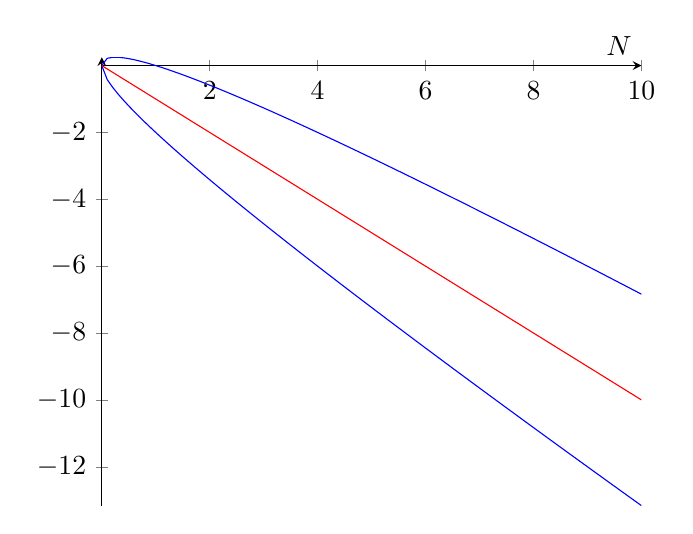
\begin{tikzpicture}
	\begin{axis}[
	axis lines = center,
	xlabel = $N$,
	]
	
	\addplot [
	domain=0:10, 
	samples=100, 
	color=blue,
	]
	{-x+x^(1/2)};
	
	
	\addplot [
	domain=0:10, 
	samples=100, 
	color=blue,
	]
	{-x-x^(1/2)};
	
	\addplot [
	domain=0:10, 
	samples=100, 
	color=red,
	]
	{-x};
	
	\end{axis}
	\end{tikzpicture}
\end{center}

\subsection*{Brownian motion}
Brownian motion is a model that describes the behaviour of particles in suspension (e.g. of dust in air, fine silt in dirty water) that have some velocity but which are constantly changing direction as they are buffeted by other particles. Their motion can be understood through a calculation similar to that for the net outcome of the binary process above, but in 3D.

The conceptual model that is often used when discussing Brownian motion is that of a \emph{random walk}. Consider a random walker who after $n$ steps is at the position ${\bf r} = (x,y,z)$. Each step is given by ${\bf s}_{n+1} = {\bf r}_{n+1}- {\bf r}_n$ and has step length $s_n$ in a random and uncorrelated direction ${\bf\hat{s}}_n$. Again (by symmetry) $\langle {\bf s}\rangle =0$. We want to find how far a particle might have gone after $N$ steps. We will define $\lambda^2= \langle {\bf s}^2\rangle$ --- the average square step-length. We write ${\bf r}_N$ for the position of the walker (or the particle) after $N$ steps, then
\begin{eqnarray*}
	\langle {\bf r}_N^2 \rangle &=& \bigg\langle \left(\sum_{n=1}^N{\bf s}_n\right)^2 \bigg\rangle\\
		&=& \bigg\langle \sum_{n=1}^N{\bf s}_n^2 +2\sum_{n=1}^{N-1}\sum_{m=n+1}^N{\bf s}_n\cdot{\bf s}_m \bigg\rangle\\
		&=& \sum\underbrace{\langle {\bf s}_n\rangle}_{=\lambda^2} + 2\sum\sum \underbrace{\langle {\bf s}_n \cdot {\bf s}_m \rangle}_{=\langle {\bf s}_n\rangle \cdot \langle{\bf s}_m \rangle=0}
\end{eqnarray*}

The first term in the expression is the mean squared step-length while the second term is zero since there is no correlation between the directions of each of the steps. Hence $\langle {\bf r}_N\rangle = N\lambda^2$ and the rms displacement is $\sqrt{N}\lambda$. If the number of steps is proportionate to the length of time that the particles move for, then we have that the mean-square displacement scales like $\sqrt{t}$. This is one of the key features of diffusive processes. 

\section*{Statistical postulates}
So far we have looked at the macroscopic properties of a thermodynamics system and at some ways of calculating properties of random processes that obey some given probability distribution. Now it is time to combine these ideas and have a first attempt at linking the microscopic behaviour of a thermodynamic system (an idealised gas) with some of its macroscopic properties.

The behaviour of a given (mechanical) system depends on both the structure of the system --- described by its equations of motion --- and on the \emph{initial conditions} of the system. Therefore, in order to describe the behaviour of the system, we need both the laws of mechanics for the system along with some statistical postulates about the initial conditions of the system. (We could also require that we know the exact initial conditions for all the particles in the system, but this is not realistic for $\mathcal{O}(10^{23})$ particles.) Different choices of the statistical postulates can lead to different behaviour (not just different states) of the system. We will look at Maxwell's postulates for the initial positions and velocities of a dilute collection of gas particles. We will see that they allow us to derive the ideal gas law from a microscopic basis.

\subsection*{An ideal gas}
We want to keep the equations of motion for our system of particles as simple as possible. We are going to assume   that our system has the following properties:
\begin{itemize}
\item We have $N$ identical  point particles, each with mass $m$, constrained in a volume $V$.
\item There are no mutual interactions --- no van der Waals effects or inter-particle forces for us!
\item The walls of the container constraining the particles are perfectly reflecting.
\item The mechanical state of the system is known when the position $\bf r$ and velocity $\bf v$ is known for each particle and these variables evolve according to Newton's laws of motion.
\end{itemize}

\subsection*{Maxwell's postulates}
We assume that the vectors describing the initial conditions of the system are randomly distributed. More specifically:
\begin{enumerate}
\item The vectors relating to each particle are independent from each other. (e.g. there is no interaction between particles when they are close.) This is generally not true for any but the most dilute systems. For such a non-interacting system, the system's state is determined when $dN=f({\bf r},{\bf v})$ is known, where $dN$ is the number of particles in a box with sides $d{\bf r}=(dx,dy,dz)$ centered on the point ${\bf r} = (x,y,z)$ and where the corresponding velocities of the particles lie within a box d${\bf v}=(dv_x,dv_y,dv_z)$ centered on ${\bf v}=(v_x,v_y,v_z)$. This relationship defines the \emph{single-particle distribution} $f({\bf r},{\bf v})$.
\item The positions ${\bf r}$ are independent of the velocities ${\bf v}$. This means we can factorise $f({\bf r},{\bf v})$ as $f({\bf r},{\bf v})$ =$f_r({\bf r})$ $f_v({\bf v})$ .
\item The density of the gas is uniform within the volume so we can write $f({\bf r}) = N/V=\rho=$ constant inside the volume (and zero outside it).
\item The velocity components are independent of each other so we can factorise $f_v$ as $f_v({\bf v})=f_x(v_x)f_y(v_y)f_z(v_z)$.
\item The distribution $f_v({\bf v})$ is isotropic in velocity space so that $f_v$ depends only on the magnitude of the velocity $|{\bf v}| = v$
\end{enumerate}

\subsection*{Equation of state}
Maxwell's postulates allow us to derive the equation of state for an ideal gas (the ideal gas law). They provide a microscopic interpretation of absolute temperature in terms of kinetic energy.

Consider a particle with velocity ${\bf v} = (v_x,v_y,v_z)$, moving from the left, that hits a wall parallel to the $yz$-plane. After impact its velocity is ${\bf v'}=(-v_x,v_y,v_z)$. Hence, the change in momentum is $\Delta {\bf p}= {\bf p'} - {\bf p} = m({\bf v'}-{\bf v}) = m(-2v_x,0,0)$.

How many such impacts occur in a given time interval $\Delta t$ on a region of the wall with area $A$? 
Take a box with a side of area $A$ on the wall and perpendicular sides of length $v_x\Delta t$. This contains the particles of velocity ${\bf v}$ that can hit the wall. The volume of the box is $Av_x\Delta t$ and the number of particles it contains is $\rho Av_x\Delta t f_v({\bf v})$, where $\rho=N/V$ is the density of all particles  and $f_v$ is the probability that a particle has velocity $\bf v$.
The total momentum $\Delta P$ transmitted to the wall is therefore
$$\Delta P =\int_0^\infty dv_x \int_{-\infty}^\infty dv_y \int_{-\infty}^\infty dv_z f_v({\bf v})\rho A\Delta t(-2m)v_x^2{\bf i}$$
where ${\bf i} =(1,0,0)$ picks out the $x$-component. I.e. integrate over the number of particles times the momentum per particle. The first integral only runs from zero since we are only interested in particles traveling towards the right, i.e. ${\bf v}>0$.

The integral above gives 
$$\Delta P = -2m\rho A\Delta t \langle v_x^2\rangle\frac12$$ where the average square velocities come from integrating over the velocity distribution and the factor of half comes from the integral over $v_x$, i.e. particles moving towards the right.
The force exerted by the gas on the wall is $F=\Delta P/\Delta t$ and pressure is force/area = $|F|/A$.
We therefore have 
\begin{equation}
	p=m\rho  \langle v_x^2\rangle.
	\label{eq1.2}
\end{equation}
 
Compare this with the classical equation of state for an ideal gas $pV=nRT$ where $n=N/N_A$, $T$ is temperature and $R=8.3 J/K$ is a constant. If we introduce the Boltzman constant $k_B = R/N_A$ and the particle density $\rho =n/V$. The ideal gas law becomes $p=\rho k_BT$. Comparing the ideal gas law with equation \ref{eq1.2} 
we find that we can relate the absolute temperature $T$ to the mean square velocities of the particles.

\section*{Phase space, Hamiltonian dynamics, and the fundamental postulate of statistical mechanics}


\subsection*{Phase space}

At a microscopic level, a thermodynamic system is comprised of $N$ particles, each with some mass $m_i$, which can interact with each other and with the boundaries of the system. (Although we are going to motivate this discussion with a thermodynamic system, everything the follows is also true for other systems where the total energy of the system is conserved --- i.e. anywhere that a Hamiltonian could show up.) If we know the positions and momenta  for each of the particles then we can completely describe the state of the system. In three dimensions, this means we must know the values for each of the $6N$ degrees of freedom; more generally, we have $2d$ d.o.f. where $d$ is the number of d.o.f. for the positions. That is the state of the system is described by a point in a $6N$ (or $2d$) dimensional phase space.
Once a point in the microscopic phase space is know, the evolution of the system is completely governed by the equations of motion for the system. These in turn are prescribed by the Hamiltonian of the system
$$H = T+U,$$
$T=$ kinetic energy, $U=$ potential energy. In general, $H$, $T$, and $U$ may all depend on both the positions and the momenta of the particles, however, for many systems we find that, conveniently, $T = \sum_i=1^N T_i$, where $T_i=\frac{{\bf p}_i^2}{2m_i}$, and the potential $U$ depends on on the positions: $U = U({\bf r}).$

If the Hamiltonian is known for a system, then the equations of motion for that system are given by
\begin{eqnarray*}
	\frac{d{\bf r}_i}{dt} &=& ~~\frac{\partial H}{\partial {\bf p}}, \\
	\frac{d{\bf p}_i}{dt} &=& -\frac{\partial H}{\partial {\bf r}}.
\end{eqnarray*}

If we write ${\bf x} = [{\bf r}^\top,{\bf p}^\top]^\top$, then we can compactly express the equations of motion as
\begin{equation}
	\frac{d{\bf x}}{dt} = f({\bf x}) = J^{-1}\nabla H({\bf x}),
\end{equation}
where
$$
	J = 
	\begin{bmatrix}
		0 & -Id\\
		Id & 0
	\end{bmatrix}.
$$
($Id$ is the identity matrix of dimension $d$.)

Given a Hamiltonian, H, and a suitable set of initial conditions ${\bf x}_0$, the evolution of the solution ${\bf x}(t)$ can be quite complicated. (Hamiltonian systems are one of the archetypal systems for studying chaotic dynamics). However, the fact that the system is Hamiltonian provides us with some additional information that can help us characterise the state of the system. For example, it is not hard to prove that a solution ${\bf x}(t)$ that satisfies $\dot{\bf x} = f({\bf x}) = J^{-1}\nabla H({\bf x}),$ ${\bf x}_0 = {\bf x}(0)$ has $H({\bf x}(t)) = H({\bf x}_0)= const.$ That is, Hamiltonian systems conserve energy along their solutions. We identify the Hamiltonian $H$ with the internal energy of the system.

Knowing that $\frac{dH}{dt}=0$, we can reduce the size of the phase space where ${\bf x}(t)$ can lie, from $2d$ d.o.f. down to $2d-1$. If we know other quantities that remain invariant over time (e.g. the total momentum of the system) then we can further reduce the size of the phase space. Strictly speaking, there are $2d-1$ invariants (AKA first integrals or constants of motion) for a Hamiltonian system. This defines a curve in the remaining 1 d.o.f. along which the solution must lie. This can be seen as a consequence of the uniqueness theorem for differential equations (think back to the 2nd year maths course on D.E.s). In reality, we typically can't find a closed form expression for most of these conserved quantities and have no idea what they might be.

It is possible that a (vanishingly) small change in the positions of the particles in phase space can lead to a large change in the state of the system and in the subsequent trajectories of the particles.
This is similar to saying that the dynamics of a Hamiltonian system can switch abruptly from regular to chaotic motion, as some parameter of the system is varied. 
Such quantities are not helpful in characterising the thermodynamics of the system.
In statistical mechanics, we are interested in the invariant quantities that only change by a little when there is a small change in the microscopic variables of the system. 
E.g. ${\bf x}\rightarrow {\bf x}+\delta {\bf x} \implies H\rightarrow H+\delta H$.

One way to phrase this is to say that we want to consider systems where thr region in phase space where the system is evolving can be (almost) completely identified, for thermodynamic purposes, by the values of a (not too large) number of observable invariant quantities.

\subsection*{Observables}
In statistical mechanics, we say that an observable is a function defined on the phase space of the system that varies smoothly with changes in the representative point of the system.
%(??? check details of QM??? This differs slightly from the situation in quantum mechanics where an observable is \emph{any} invariant quantity of the system (AKA first integral, AKA constant of motion). I.e. any operator that commutes with the Hamiltonian)

The kinetic energy $\sum_i \frac{p_i}{2m_i}$ is an observable, while the function $\Theta = \prod_i \theta(r_0^2-r_i^2)$, where $\theta(x)$ is the Heaviside function, is not, since an arbitrarily small change in a position $r_i$ can lead to a finite change in $\Theta.$

Other examples of (thermodynamic) observables include the internal energy $E$ (i.e. the Hamiltonian) and the number of particles in the system ($N = \int d{\bf r}\sum\delta({\bf r}-{\bf r}_i)$).
It turns out that the entropy $S=S(X_0=E=H,X_1,\ldots,X_r)$ is also an observable. However, we don't yet have a way to express the entropy --- the extensive variable of a thermodynamic system --- as a function of the microscopic state of the system and its equations of motion. To do so, we are going to invoke the fundamental postulate of statistical mechanics.

\subsection*{The fundamental postulate of statistical mechanics}
The fundamental postulate expresses the entropy $S$ as a function of the accessible volume of the phase space of a dynamical system. I.e. that part of the phase space where the observables have values that are compatible with a specific thermodynamic state.

Assume that the thermodynamic state of a system is determined by the extensive variables $X_1,\ldots,X_r$ and that each of the $X_i$ can be expressed as a function over the microscopic phase space; I.e. $X_i = X_i({\bf x})$.
The region of phase space that is accessible is defined by the value of $X = (X_1,\ldots,X_r)$. Well, almost; we actually also allow for small discrepancies $\epsilon_i,~~i=1,\ldots,r$ to account for the effect of any non-extensive terms.

We denote the region of phase space in which the observable $X_i$ have the specific values that match the thermodynamic state as $\Gamma$ and we denote the corresponding phase space volume $\text{vol}(\Gamma)=\Omega$. Then the fundamental postulate of thermodynamics states that
\begin{equation}
	S = k_B\ln(\Omega),
	\label{eqS}
\end{equation}
where $S$ is the thermodynamic entropy, $K_B$ is Boltzmann's constant ($K_B = 1.384\times10^{-23}$J/K) and the equality should be interpreted as meaning ``is equal, up to terms of size $\epsilon_i$''. The accessible phase space volume $\Omega$ measures the amount of the phase space available to the microscopic system while it is in this macroscopic state. If the system had only discrete micro-states, then we could simply count the number of micro-states that correspond to the same macro-state. We therefore identify $\Omega$ with the partition function.

\subsection*{Symplectic transformations and phase space area preservation}
Why is phase space so important in the formulation of entropy? To understand this we are going to look closer at some of the properties that being Hamiltonian impose on a system, including the choice of coordinate system.

We saw earlier that the equations of motion for a time-independent Hamiltonian system can be written as$ \frac{d{\bf x}}{dt} = f({\bf x}) = J^{-1}\nabla H({\bf x})$. This Hamiltonian form is not preserved by arbitrary coordinate transformations; it \emph{is} preserved by \emph{symplectic} transformations.

{\bf Definition:} A linear transformation $A: \mathbb{R}^{2d}\rightarrow\mathbb{R^{2d}}$ is said to be symplectic if it satisfies
$$ A^\top J A = J.$$
For a non-linear transformation $\mathcal{A}$, we replace $A$ above with its jacobian $D\mathcal{A}$.

An alternative, but equivalent, definition of a symplectic transformation --- and one that will turn out to be useful in a bit --- borrows some tools from differential geometry. (No prior experience with differential geometry is assumed.)

{\bf Definitions:} A symplectic transformation is a diffeomorphisim (a smooth, invertible mapping between manifolds) $f:\mathbb{R}^2d\rightarrow\mathbb{R}^2d$, with coordinates $r$ and $p$, which preserves the symplectic two-form $\omega$ (an anti-symmetric, bilinear form) that acts on pairs of vectors and gives the sum of the oriented areas that they define. In two dimensions, this is the area of the parallelogram spanned by the two vectors.

More explicitly,
\begin{equation*}
	\omega(u,v) = u^\top Jv = \sum_{i=1}^d u_{p_i} v_{r_i} - u_{r_i} v_{p_i}.
\end{equation*}

At this point it is necessary to introduce a (potentially) new concept --- the flow map of a vector field. The flow $\varphi_{t,f}({\bf x})$ of a Hamiltonian system is a function that maps a point ${\bf x}^*$ in the phase space of the system with equations of motion $\dot{\bf x} = f({\bf x}) =J^{-1}\nabla H({\bf x})$ forward by time $t$. I.e. for any $f({\bf x})$ and ${\bf x}_0$, $\varphi_{t,f}({\bf x}_0)$ gives the solution to $\dot{\bf x}=f({\bf x})$ at time $t$.

{\bf Theorem:} If the Hamiltonian $H({\bf x})$ is a twice differentiable function on some neighbourhood of $\mathbb{R}^2d$, then the time-$t$ flow map $\varphi_{t,f}({\bf x}_0)$ of the Hamiltonian vector field is a symplectic map for all $t$.
{\bf Proof:} We will show that $\omega(u,v)=u^\top J v$ is constant along solutions of $\dot{\bf x} = J^{-1}\nabla H({\bf x})$.

The tangent vector $u(t) = \frac{\partial \varphi_t}{\partial {\bf x}_0}({\bf x}_0)u(0)$ satisfies $\frac{du}{dt} = J^{-1}\nabla^2H({\bf x}(t))u(t)$ and the tangent vector $v(t)$ satisfies a similar expression. Now we can calculate the time derivative of $\omega(u,v)$.
\begin{eqnarray*}
	\frac{d}{dt}\omega(u,v) &=& \dot{u}^{\top}Jv+u^\top J\dot{v}\\
		&=& (J^{-1}\nabla^2Hu)^\top Jv + u^\top JJ^{-1}\nabla^2Hv\\
		&=& 0
\end{eqnarray*}
since $J^{-\top}J=-I$ and $JJ^{-1} = I$.

I.e. as the system evolves according to its equations of motion, it always preserves the area for $d=1$, or the sum of the oriented areas for $d \geq2$.


\subsection*{Liouville's theorem and preservation of phase space volume}
We are now in a position to prove that the flow of a Hamiltonian system preserves phase space volume. That is, for every bounded, open set $A\subset\mathcal{R}^{2d}$ and every $t$ for which $\varphi_{t,f}({\bf x})$ exists
$$\text{Vol}(\varphi_{t,f}(\Gamma))=Vol(\Gamma)$$
where $f=J^{-1}\nabla H$ and $Vol(\Gamma) = \int_{\Gamma}d{\bf x}$.

To prove this, we will actually prove a slightly more general case: the flow of a differential equation $\dot{\bf x}=f({\bf x})$ in $\mathbb{R}^n$ is volume preserving if and only if it is divergence free. I.e. $\nabla\cdot f=0$.

But first, why do we care about preservation of phase space volume? The fundamental postulate of statistical mechanics, $S=k_B\ln(\Omega)$ related the entropy of a system to the volume of the part of the phase space accessible to that system when it is in that particular thermodynamic state. We would like to be sure that this quantity doesn't vary too much over time as the microscopic system evolves, according to the Hamiltonian equations of motion. Although the microscopic system might be in continuous motion, the trajectories of the particles it is comprised of are such that the extensive variables which characterise the macroscopic state of the system are (almost) constant. I.e. there is no change in entropy, no heat flow, no work done while the system is at equilibrium. This is reassuring --- it says that disorder doesn't increase unless something happens.

{\bf Proof: volume preservation:}
The Jacobian of the flow map $\varphi_{t,f}({\bf x}_0)$ defines the matrix function $X(t)=D\varphi_{t,f}({\bf x}_0)$. The volume of the shape spanned by the columns of $X$ is given by $\det(X)$, and $X(t)$ is a solution of the equation
$$
\dot{X}=A(t)X(t),\qquad X(0)=I,
$$
where $A(t):=Df({\bf x}(t))$ denotes the Jacobian of $f({\bf x}(t))$ evaluated at ${\bf x}(t)=\varphi_{t,f}({\bf x}_0)$. To show that the volume defined by $X$ is constant we use  the Abel-Liouville-Jacobi-Ostrogradskii identity to find the time derivative of $\det X$:
$$
\frac{d}{dt}\det X(t)=\text{trace} A(t)\cdot\det X(t).
$$
Since $A(t)=Df({\bf x}(t))$ we have $\text{trace} A(t)=\sum_i\frac{\partial f_i}{\partial {\bf x}_i}({\bf x}(t))=\nabla\cdot f({\bf x}(t))$ and therefore $\det X(t)=\det X(0)=1$ if and only if $\nabla\cdot f({\bf x})=0.$

\subsection*{Recommended reading}
This section has mostly followed the first half of chapter 3 of \emph{Statistical Mechanics in a Nutshell}. However, some of the significance of Hamiltonian systems is lost in SMiaN, so I've supplemented it with more substantive (mathematically oriented) details from \emph{Geometric Numerical Integration} by E. Hairer, Ch. Lubich and G. Wanner (Springer, 2006) --- one of the best books on (the numerics of) Hamiltonian dynamical systems and a personal favourite.



\end{document}
